%%%%%%%%%%%%%%%%%%%%%%%%%%%%%%%%%%%%%%%%%
% Journal Article
% LaTeX Template
% Version 1.4 (15/5/16)
%
% This template has been downloaded from:
% http://www.LaTeXTemplates.com
%
% Original author:
% Frits Wenneker (http://www.howtotex.com) with extensive modifications by
% Vel (vel@LaTeXTemplates.com)
%
% License:
% CC BY-NC-SA 3.0 (http://creativecommons.org/licenses/by-nc-sa/3.0/)
%
%%%%%%%%%%%%%%%%%%%%%%%%%%%%%%%%%%%%%%%%%

%----------------------------------------------------------------------------------------
%	PACKAGES AND OTHER DOCUMENT CONFIGURATIONS
%----------------------------------------------------------------------------------------

\documentclass[twoside,twocolumn]{article}

\usepackage{blindtext} % Package to generate dummy text throughout this template 

\usepackage[sc]{mathpazo} % Use the Palatino font
\usepackage[T1]{fontenc} % Use 8-bit encoding that has 256 glyphs
\linespread{1.05} % Line spacing - Palatino needs more space between lines
\usepackage{microtype} % Slightly tweak font spacing for aesthetics

\usepackage{graphicx} % Importing because I want to see pictures and images in the document

\usepackage[english]{babel} % Language hyphenation and typographical rules

\usepackage[hmarginratio=1:1,top=32mm,columnsep=20pt]{geometry} % Document margins
\usepackage[hang, small,labelfont=bf,up,textfont=it,up]{caption} % Custom captions under/above floats in tables or figures
\usepackage{booktabs} % Horizontal rules in tables

\usepackage{lettrine} % The lettrine is the first enlarged letter at the beginning of the text

\usepackage{enumitem} % Customized lists
\setlist[itemize]{noitemsep} % Make itemize lists more compact

\usepackage{abstract} % Allows abstract customization
\renewcommand{\abstractnamefont}{\normalfont\bfseries} % Set the "Abstract" text to bold
\renewcommand{\abstracttextfont}{\normalfont\small\itshape} % Set the abstract itself to small italic text

\usepackage{titlesec} % Allows customization of titles
\renewcommand\thesection{\Roman{section}} % Roman numerals for the sections
\renewcommand\thesubsection{\roman{subsection}} % roman numerals for subsections
\titleformat{\section}[block]{\large\scshape\centering}{\thesection.}{1em}{} % Change the look of the section titles
\titleformat{\subsection}[block]{\large}{\thesubsection.}{1em}{} % Change the look of the section titles

\usepackage{fancyhdr} % Headers and footers
\pagestyle{fancy} % All pages have headers and footers
\fancyhead{} % Blank out the default header
\fancyfoot{} % Blank out the default footer
\fancyhead[C]{Design Plan $\bullet$ April 2022} % Custom header text
\fancyfoot[ROLE]{\thepage} % Custom footer text

\usepackage{titling} % Customizing the title section

\usepackage{hyperref} % For hyperlinks in the PDF

\usepackage{biblatex} %Imports biblatex package
\usepackage{csquotes}
\addbibresource{wilt.bib} %Import the bibliography file

%----------------------------------------------------------------------------------------
%	TITLE SECTION
%----------------------------------------------------------------------------------------

\setlength{\droptitle}{-4\baselineskip} % Move the title up

%\pretitle{\begin{center}\Huge\bfseries} % Article title formatting
%\posttitle{\end{center}} % Article title closing formatting
\title{Scavenger Hunt Design Plan} % Article title
\author{%
\textsc{Henry Wilt} \\[1ex]%\thanks{A thank you or further information}  % Your name
\normalsize Ursinus College \\ % Your institution
\normalsize \href{mailto:hewilt@ursinus.edu}{hewilt@ursinus.edu} % Your email address
\and % Uncomment if 2 authors are required, duplicate these 4 lines if more
\textsc{Marcos Maciel} \\[1ex] % Second author's name \thanks{Corresponding author}
\normalsize Ursinus College \\ % Second author's institution
\normalsize \href{mailto:mamaciel@ursinus.edu}{mamaciel@ursinus.edu} % Second author's email address
\and % Uncomment if 2 authors are required, duplicate these 4 lines if more
\textsc{Arthur Artene} \\[1ex] % Second author's name \thanks{Corresponding author}
\normalsize Ursinus College \\ % Second author's institution
\normalsize \href{mailto:arartene@ursinus.edu}{arartene@ursinus.edu} % Second author's email address
\and % Uncomment if 2 authors are required, duplicate these 4 lines if more
\textsc{Alex Crocamo} \\[1ex] % Second author's name \thanks{Corresponding author}
\normalsize Ursinus College \\ % Second author's institution
\normalsize \href{mailto:alcrocamo@ursinus.edu}{alcrocamo@ursinus.edu} % Second author's email address
}
\date{\today} % Leave empty to omit a date
\renewcommand{\maketitlehookd}{%

% ----------------------------------------------------------
% Abstract!!
\begin{abstract}
\noindent %\blindtext % Dummy abstract text - replace \blindtext with your abstract text
The purpose for our Design Plan is to show what we want we want to do for the final project, being our goal for having a working Scavenger Hunt that First Years can use to find their way around Campus. What our Affordances and Signifiers are; along with who are our Stakeholders are or could be for the project. The project is made for our CS474 Course, Human Computer Interaction\cite{wmonganweb}.
\end{abstract}
}

%----------------------------------------------------------------------------------------

\begin{document}

% Print the title
\maketitle

%----------------------------------------------------------------------------------------
%	ARTICLE CONTENTS
%----------------------------------------------------------------------------------------

\section{What we want to do}
% Type in this section for words to show up in the doc
\par We propose to make a scavenger hunt for First Years/Transfer students at Ursinus. Each Building/location will be an achievement to get during the scavenger hunt. Once the scavenger hunt is completed, you get a time of how long it took you to find all the locations. This will be made up in an app with the end goal of integrating it with the MobileU app.


\subsection{Achievements}

\includegraphics[scale=0.25]{Achievements/Bear Legend.png}\footnote{Bear Legend Achievement}

\includegraphics[scale=0.25]{Achievements/Bomberger.png}\footnote{Bomberger Achievement}
\par The goal for the Scavenger Hunt to find all the building and collecting all the achievements in the Hunt. For example the Bomberger Achievement is gained through scanning and finding Bomberger Hall. While the Bear Legend Achievement is gained through getting all the Achievements\cite{achievements} in the Scavenger Hunt.


%------------------------------------------------

\section{Our Affordances and Signifiers}
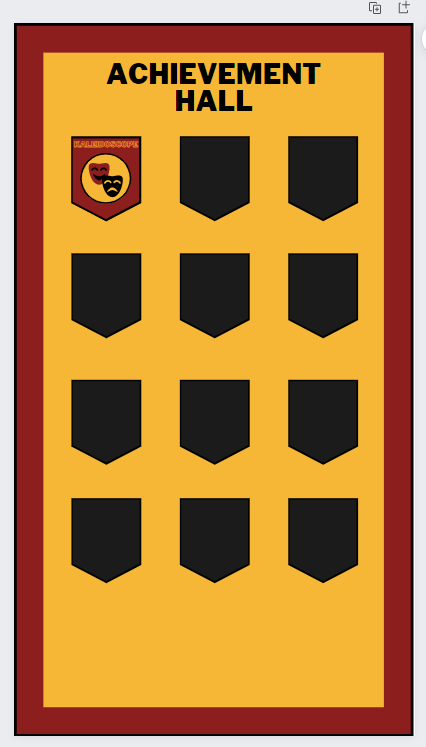
\includegraphics[scale=0.25]{Achievements/Achievement_Page.png}\footnote{Achievement Page}
\par During our project we will look into what the Affordances and Signifiers are. If their are undesirable ones then we will try and fix them by using our stakeholders to test our software. Our interface will pretty simple to follow along with the main menu having readable text and easy follow along buttons. Where one will take you to the Scavenger Hunt, another to the Achievement Page, and the Leaderboard.

%What is an Affordance?
%What is a Signifier?

%------------------------------------------------

\section{About our Stakeholders}
\par There are a couple of Stakeholders that we could think of as a group. Starting off with The College (Ursinus College) as the being the biggest Stakeholder as they will be using to teach the First Years about finding their way around the campus in a safe and speedy manner. As First Years and Transfer Students can get themselves lost around campus or not know where or what each building is, The College would be very interested in fixing that problem. Another Stakeholder would be the actual First Year or Transfer Student as they are trying to find themselves around campus and would like to know where to go and not get lost. As they are the ones who interact the most with the Scavenger Hunt, we need their feedback to make sure that it is; one not that complex to use or download, and two have them actually want to/ find the time to use the Hunt as a resource to find their way around the campus.

%------------------------------------------------

% if you want to add another section use the /section{}
\section{Conclusion}
In this Design Plan, we talked about what we propose to do for the project, our stakeholders, a little bit about the design of the app, and a little about the Achievements that are planned. The Scavenger Hunt should help First Years and Transfer Students get around campus. Our main two stakeholders are The College and the Students using the app. 


%----------------------------------------------------------------------------------------
%	REFERENCE LIST
%----------------------------------------------------------------------------------------

\printbibliography %Prints bibliography

%----------------------------------------------------------------------------------------

\end{document}
